\chapter{Phase shift transducer}
\section{Theory and related work} \label{sec:literature_linear}
This circuit comprises the use of voltage comparators used as zero crossing detectors, a XOR gate as well as a low pass filter. An operational amplifier comparator is a circuit that compares one analogue voltage level with a reference voltage and outputs a signal based on this voltage comparison, this operational amplifier is used in open loop mode and switches between its two saturated states. %https://www.electronics-tutorials.ws/opamp/op-amp-comparator.html
A XOR gate is a digital logic gate with two or more inputs and one output and performs the exclusive disjunction between these input voltage levels. %https://logic.ly/lessons/xor-gate/ 
A low pass filter is a circuit that allows signals with a frequency lower than that of the cut-off frequency to pass through it, and blocks all frequencies higher than the cut off frequency. A single pole low pass filter consisting of a resistor and a capacitor can be used to smooth a PWM signal into an analogue voltage level.
%https://www.allaboutcircuits.com/technical-articles/turn-your-pwm-into-a-dac/
\section{Design} \label{sec:design_linear}
%http://sound-au.com/appnotes/an005.htm
The first step in determining the phase difference between two sinusoidal waves is to determine when each of these sinusoidal signals pass through the zero axis, and more specifically when each sinusoid is positive. This was implemented by using an operational amplifier comparator as a zero crossing detector, in this configuration the input voltage was applied at the non inverting pin and the reference input was applied at the inverting input pin and was set to \SI{100}{\milli \volt}. It was found that a ground reference produced an unstable and unpredictable output due to noise under no load conditions. The operational amplifier used for this design was the TLC2272, this chip was chosen due to its rail to rail capabilities and due to space constraints as it contained two operational amplifiers per chip. Both of the comparators were used in single supply mode, thus its two saturated states corresponded to \SI{0}{\volt} and \SI{5}{\volt} respectively, this meant that if an input signal was positive the comparator's output would be \SI{5}{\volt}, and if the signal was less than the reference signal the output would be \SI{0}{\volt}. The input voltage to the zero crossing detector for the voltage level was taken as the output from the voltage divider network in Figure \ref{fig:voltagepeakdetector.pdf}, labelled as v\_meas, and the input voltage to the zero crossing detector for the current level was taken as the output from the gain stage in Figure \ref{fig:currentpeakdetector.pdf}, labelled as i\_meas. Both of these input signals had a maximum voltage of \SI{5}{\volt} and thus were within the limits of the differential mode input of the operational amplifiers. Given that it was now determined when each sinusoidal input crossed the zero axis the phase delay between these signals could now be found. This was done by using a logical XOR gate that would output a logical high for the duration that the two sinusoids were out of phase. Since the input signals are periodic the output of the XOR gate would be a pulse width modulated signals with a varying duty cycle depending on how out of phase the two input signals are.
%https://www.allaboutcircuits.com/technical-articles/turn-your-pwm-into-a-dac/
To turn this PWM signal into an analogue signal a simple digital to analogue converter was implemented by using a single pole RC low pass filter. The   

\begin{align}
    f_{cut-off}=\frac{1}{2\pi RC}
   \label{eq:opampgain}
\end{align}

\begin{figure}[h!]
    \centering
    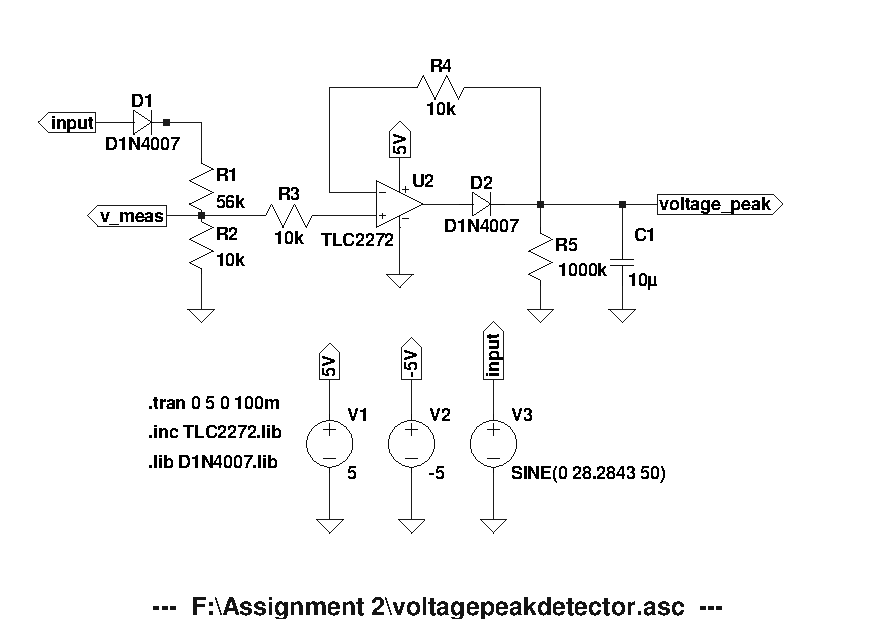
\includegraphics[width = 0.65\linewidth]{Figures/voltagepeakdetector.pdf}
        \caption{Phase Shift Detector Diagram}
    \label{fig:phaseshiftdetector.pdf}
\end{figure}

\section{Simulation} \label{sec:simulation_linear}

\section{Measurements} \label{sec:measurements_linear}








